\chapter{Tuples | 元组}
\label{tuplechap}

This chapter presents one more built-in type, the tuple, and then
shows how lists, dictionaries, and tuples work together.
I also present a useful feature for variable-length argument lists,
the gather and scatter operators.

本章节介绍另一个内建的类型 --- 元组,然后向您展示列表、字典和元组如何在一起使用。我也会展示一个有用的功能......

One note: there is no consensus on how to pronounce ``tuple''.
Some people say ``tuh-ple'', which rhymes with ``supple''.  But
in the context of programming, most people say ``too-ple'', which
rhymes with ``quadruple''.


\section{Tuples are immutable | 元组的不可变性}
\index{tuple}
\index{type!tuple}
\index{sequence}

A tuple is a sequence of values.  The values can be any type, and
they are indexed by integers, so in that respect tuples are a lot
like lists.  The important difference is that tuples are immutable.
\index{mutability}
\index{immutability}

元组是一组值的序列。  其中的 \emph{值}可以是任意类型,使用整数索引其位置,因此元组与列表非常相似。  而重要的不同之处在于元组的不可变性。

Syntactically, a tuple is a comma-separated list of values:

语法上,元组是用逗号隔开的值的列表:

\begin{lstlisting}
>>> t = 'a', 'b', 'c', 'd', 'e'
\end{lstlisting}
%
Although it is not necessary, it is common to enclose tuples in
parentheses:

尽管不是必须,通常我们在给元组赋值时会用括号把元素封装起来:

\index{parentheses!tuples in}

\begin{lstlisting}
>>> t = ('a', 'b', 'c', 'd', 'e')
\end{lstlisting}
%
To create a tuple with a single element, you have to include a final
comma:

使用单一元素建立元组时,你需要在结尾使用一个逗号:

\index{singleton}
\index{tuple!singleton}

\begin{lstlisting}
>>> t1 = 'a',
>>> type(t1)
<class 'tuple'>
\end{lstlisting}
%
A value in parentheses is not a tuple:

括号中仅包含元素(而没有使用逗号结尾)的对象其实不是元组:

\begin{lstlisting}
>>> t2 = ('a')
>>> type(t2)
<class 'str'>
\end{lstlisting}
%
Another way to create a tuple is the built-in function {\tt tuple}.
With no argument, it creates an empty tuple:
\index{tuple function}
\index{function!tuple}

另一个建立元组的方法是使用内建函数 \lstinline{tuple}。 在没有参数传递时它会产生一个空元组。

\begin{lstlisting}
>>> t = tuple()
>>> t
()
\end{lstlisting}

%
If the argument is a sequence (string, list or tuple), the result
is a tuple with the elements of the sequence:



\begin{verbatim}
>>> t = tuple('lupins')
>>> t
('l', 'u', 'p', 'i', 'n', 's')
\end{verbatim}
%
Because {\tt tuple} is the name of a built-in function, you should
avoid using it as a variable name.

因为\lstinline{tuple}是内建函数名,所以应该避免将它用于变量名。


Most list operators also work on tuples.  The bracket operator
indexes an element:

列表的大多数操作同样也适用于元组。 例如使用方括号索引一个元素:

\index{bracket operator}
\index{operator!bracket}

\begin{lstlisting}
>>> t = ('a', 'b', 'c', 'd', 'e')
>>> t[0]
'a'
\end{lstlisting}
%
And the slice operator selects a range of elements.

切片操作可以选取一个范围内的元素:
\index{slice operator}
\index{operator!slice}
\index{tuple!slice}
\index{slice!tuple}

\begin{lstlisting}
>>> t[1:3]
('b', 'c')
\end{lstlisting}
%
But if you try to modify one of the elements of the tuple, you get
an error:

但是,如果你试图元组中的一个元素,你将会得到错误提示:

\index{exception!TypeError}
\index{TypeError}
\index{item assignment}
\index{assignment!item}

\begin{lstlisting}
>>> t[0] = 'A'
TypeError: object doesn't support item assignment
\end{lstlisting}
%
Because tuples are immutable, you can't modify the elements.  But you
can replace one tuple with another:

因为元组是不可变的,您无法改变其中的元素。 但是您可以使用其他元组替换现有元组:

\begin{lstlisting}
>>> t = ('A',) + t[1:]
>>> t
('A', 'b', 'c', 'd', 'e')
\end{lstlisting}
%
This statement makes a new tuple and then makes {\tt t} refer to it.

这个语句产生了一个新元组,并且将它赋给了原先的元组\lstinline{t}。

The relational operators work with tuples and other sequences;
Python starts by comparing the first element from each
sequence.  If they are equal, it goes on to the next elements,
and so on, until it finds elements that differ.  Subsequent
elements are not considered (even if they are really big).

关系型操作也适用于元组和其他序列;Python 会首先比较序列中的第一个元素,如果它们相同就会去比较下一组元素,以此往复,直至比值不同。 其后的元素(即便是差异很大)也不会再参与比较。

\index{comparison!tuple}
\index{tuple!comparison}

\begin{lstlisting}
>>> (0, 1, 2) < (0, 3, 4)
True
>>> (0, 1, 2000000) < (0, 3, 4)
True
\end{lstlisting}


\section{Tuple assignment | 元组赋值}
\label{tuple.assignment} \index{tuple!assignment} \index{assignment!tuple}
\index{swap pattern} \index{pattern!swap}

It is often useful to swap the values of two variables.
With conventional assignments, you have to use a temporary
variable.  For example, to swap {\tt a} and {\tt b}:

两个变量互换值的操作通常很有用。 传统的,你需要使用一个临时变量。 例如为了交换\lstinline{a}和\lstinline{b}:

\begin{lstlisting}
>>> temp = a
>>> a = b
>>> b = temp
\end{lstlisting}
%
This solution is cumbersome; {\bf tuple assignment} is more elegant:

这个方法很繁琐;通过{\bf 元组赋值}的操作来实现则优雅许多:

\begin{lstlisting}
>>> a, b = b, a
\end{lstlisting}
%
The left side is a tuple of variables; the right side is a tuple of
expressions.  Each value is assigned to its respective variable.
All the expressions on the right side are evaluated before any
of the assignments.

等号左侧是两个变量构成的元组;右侧则是用于给元组赋值的表达式。  每个值都被赋给了要互换的对应变量。变量被重新赋值前,右侧的表达式会被优先操作。

The number of variables on the left and the number of
values on the right have to be the same:

使用元组赋值,左右的变量数必须相同:

\index{exception!ValueError}
\index{ValueError}

\begin{lstlisting}
>>> a, b = 1, 2, 3
ValueError: too many values to unpack
\end{lstlisting}
%
More generally, the right side can be any kind of sequence
(string, list or tuple).  For example, to split an email address
into a user name and a domain, you could write:

一般说来,元组赋值的右侧表达式可以是任意类型(字符串、列表或者元组)的序列。 例如, 为了将一个电子邮件地址分割成用户名和域名, 你可以写:

\index{split method}
\index{method!split}
\index{email address}

\begin{lstlisting}
>>> addr = 'monty@python.org'
>>> uname, domain = addr.split('@')
\end{lstlisting}
%
The return value from {\tt split} is a list with two elements;
the first element is assigned to {\tt uname}, the second to
{\tt domain}.

\lstinline{split}函数返回的对象是一个具有两个元素的列表;第一个元素被赋给了\lstinline{uname}的变量,第二个被赋给了\lstinline{domain}。

\begin{lstlisting}
>>> uname
'monty'
>>> domain
'python.org'
\end{lstlisting}
%

\section{Tuples as return values | 元组作为返回值}
\index{tuple} \index{value!tuple} \index{return value!tuple}
\index{function, tuple as return value}

Strictly speaking, a function can only return one value, but
if the value is a tuple, the effect is the same as returning
multiple values.  For example, if you want to divide two integers
and compute the quotient and remainder, it is inefficient to
compute {\tt x/y} and then {\tt x\%y}.  It is better to compute
them both at the same time.

严格地说,一个函数只能返回一个值,当如果这个值是元组,其效果等同于返回多个值。 例如,你想对两个整数做除法,计算出商和余数,先后计算出\lstinline{x/y}和\lstinline{x%y}是很低效的。最好的方法就是同时计算出它们。
\index{divmod}

The built-in function {\tt divmod} takes two arguments and
returns a tuple of two values, the quotient and remainder.
You can store the result as a tuple:

内建函数\lstinline{divmod}接受两个参数,并且返回具有两个值的元组 --- 商和余数。您可以使用元组来存储返回值:

\begin{lstlisting}
>>> t = divmod(7, 3)
>>> t
(2, 1)
\end{lstlisting}
%
Or use tuple assignment to store the elements separately:

或者使用元组赋值来分别存储它们:

\index{tuple assignment}
\index{assignment!tuple}

\begin{lstlisting}
>>> quot, rem = divmod(7, 3)
>>> quot
2
>>> rem
1
\end{lstlisting}
%
Here is an example of a function that returns a tuple:

另一个返回元组作为结果的函数例子:

\begin{lstlisting}
def min_max(t):
    return min(t), max(t)
\end{lstlisting}
%
{\tt max} and {\tt min} are built-in functions that find
the largest and smallest elements of a sequence.  \verb"min_max"
computes both and returns a tuple of two values.

\lstinline{max} 和 \lstinline{min} 是用于找出一组元素序列中最大值和最小值的内建函数,\lstinline{min_max}函数同时计算出它们并组装成元组返回结果。
\index{max function} \index{function!max}
\index{min function} \index{function!min}


\section{Variable-length argument tuples | 可变长度参数元组}
\label{gather}
\index{variable-length argument tuple} \index{argument!variable-length tuple}
\index{gather} \index{parameter!gather} \index{argument!gather}

Functions can take a variable number of arguments.  A parameter
name that begins with {\tt *} {\bf gathers} arguments into
a tuple.  For example, {\tt printall}
takes any number of arguments and prints them:

函数可以同时接受多个参数。 以 {\bf *} 开头的定义参数可以将输入的参数 \emph{汇集}到一个元组中。 例如 \lstinline{printall} 可以接受任意数量的参数,并且打印出来:

\begin{lstlisting}
def printall(*args):
    print(args)
\end{lstlisting}
%
The gather parameter can have any name you like, but {\tt args} is
conventional.  Here's how the function works:

汇集的形参可以使用任意名字, 传统上我们使用\lstinline{args}. 以下显示了这个函数的调用效果:

\begin{lstlisting}
>>> printall(1, 2.0, '3')
(1, 2.0, '3')
\end{lstlisting}
%
The complement of gather is {\bf scatter}.  If you have a
sequence of values and you want to pass it to a function
as multiple arguments, you can use the {\tt *} operator.
For example, {\tt divmod} takes exactly two arguments; it
doesn't work with a tuple:

\emph{离散}{\bf scatter}是汇集的补充。 如果你有一个值的序列,并且希望
将其作为多个参数传递给一个函数,你可以使用运算符\lstinline{*}。
例如,\lstinline{divmod} 需要接受两个实参;一个元组则无法作为参数传递进去:

\index{scatter} \index{argument scatter} \index{TypeError}
\index{exception!TypeError}

\begin{lstlisting}
>>> t = (7, 3)
>>> divmod(t)
TypeError: divmod expected 2 arguments, got 1
\end{lstlisting}
%
But if you scatter the tuple, it works:

但是如果您将这个元组打散,它就可以被传递进函数:

\begin{lstlisting}
>>> divmod(*t)
(2, 1)
\end{lstlisting}

%
Many of the built-in functions use
variable-length argument tuples.  For example, {\tt max}
and {\tt min} can take any number of arguments:

多数内建函数使用可变长度参数元组。 例如,\lstinline{max} 和 \lstinline{min} 可以取任意数量的参数。

\index{max function} \index{function!max}
\index{min function} \index{function!min}

\begin{lstlisting}
>>> max(1, 2, 3)
3
\end{lstlisting}
%
But {\tt sum} does not.

但是求和\lstinline{sum}操作并不如此:
\index{sum function} \index{function!sum}

\begin{lstlisting}
>>> sum(1, 2, 3)
TypeError: sum expected at most 2 arguments, got 3
\end{lstlisting}
%
As an exercise, write a function called {\tt sumall} that takes any number
of arguments and returns their sum.

您可以尝试写一个叫做 \lstinline{sumall}的函数作为练习,使它能够接受任何数量的传参并返回它们的和。

\section{Lists and tuples | 列表和元组}
\index{zip function} \index{function!zip}

{\tt zip} is a built-in function that takes two or more sequences and
returns a list of tuples where each tuple contains one
element from each sequence.  The name of the function refers to
a zipper, which joins and interleaves two rows of teeth.

\lstinline{zip} 是一个内建函数,用于将两个或多个序列组装成包含元组的列表返回出来,每个元组包含了各个序列中相对位置的一个元素。这个函数的起名来源于名词拉链(zipper),形象的显示年对应两列对应位置的牙齿组合起来。

This example zips a string and a list:

下面例子显示了组合字符串和列表操作:

\begin{lstlisting}
>>> s = 'abc'
>>> t = [0, 1, 2]
>>> zip(s, t)
<zip object at 0x7f7d0a9e7c48>
\end{lstlisting}
%
The result is a {\bf zip object} that knows how to iterate through
the pairs.  The most common use of {\tt zip} is in a {\tt for} loop:

输出的结果是一个可以通过每个内在的元组对进行迭代的 \lstinline{zip} 对象。 \lstinline{zip}函数最常见用法就是基于\lstinline{for}循环的迭代遍历:

\begin{lstlisting}
>>> for pair in zip(s, t):
...     print(pair)
...
('a', 0)
('b', 1)
('c', 2)
\end{lstlisting}

%
A zip object is a kind of {\bf iterator}, which is any object
that iterates through a sequence.  Iterators are similar to lists in some
ways, but unlike lists, you can't use an index to select an element from
an iterator.

\lstinline{zip}对象是一个友善的\textbf{迭代器},后者是指任何一种能够按照某个序列迭代的对象。 迭代器在某些方面与列表非常相似, 不同之处在于你无法通过索引来选择迭代其中的某个元素。
\index{iterator} \index{迭代器}

If you want to use list operators and methods, you can
use a zip object to make a list:

如果你想对\lstinline {zip}对象使用列表的操作和方法,你可以通过\lstinline {zip}对象创造一个列表:

\begin{lstlisting}
>>> list(zip(s, t))
[('a', 0), ('b', 1), ('c', 2)]
\end{lstlisting}

%
The result is a list of tuples; in this example, each tuple contains
a character from the string and the corresponding element from
the list.

结果就是产生了一个包含若干元组的列表;在这个例子中,每个元组又包含了字符串中的一个字符和列表\lstinline {t} 中对应的一个元素。
\index{list!of tuples}

If the sequences are not the same length, the result has the
length of the shorter one.

如果用于创建\lstinline{zip}的序列长度不一,返回的对象的长度以最短序列的长度为准。

\begin{lstlisting}
>>> list(zip('Anne', 'Elk'))
[('A', 'E'), ('n', 'l'), ('n', 'k')]
\end{lstlisting}
%
You can use tuple assignment in a {\tt for} loop to traverse a list of
tuples:

您可以通过元组赋值在\lstinline{for}循环中遍历包含元组的列表:
\index{traversal} \index{tuple assignment} \index{assignment!tuple}

\begin{lstlisting}
t = [('a', 0), ('b', 1), ('c', 2)]
for letter, number in t:
    print(number, letter)
\end{lstlisting}
%
Each time through the loop, Python selects the next tuple in
the list and assigns the elements to {\tt letter} and
{\tt number}.  The output of this loop is:

循环中的每次执行, Python 会选择列表中的下一个元组,并将其内容赋给 \lstinline{letter} 和 \lstinline{number}。因此循环打印的输出会是这样:
\index{loop}

\begin{lstlisting}
0 a
1 b
2 c
\end{lstlisting}

%
If you combine {\tt zip}, {\tt for} and tuple assignment, you get a
useful idiom for traversing two (or more) sequences at the same
time.  For example, \verb"has_match" takes two sequences, {\tt t1} and
{\tt t2}, and returns {\tt True} if there is an index {\tt i}
such that {\tt t1[i] == t2[i]}:

如果将zip、for和元组赋值结合起来使用,您会得出一个有用的惯用方法用来
同时遍历两个(甚至多个)序列。 如下例,\lstinline{has_match} 接受两个序列,\lstinline{t1}和\lstinline{t2},并返回一个真值\lstinline{True}如果存在满足判别式 \lstinline{t1[i] == t2[i]}的索引\lstinline {i}:
\index{for loop}

\begin{lstlisting}
def has_match(t1, t2):
    for x, y in zip(t1, t2):
        if x == y:
            return True
    return False
\end{lstlisting}

%
If you need to traverse the elements of a sequence and their
indices, you can use the built-in function {\tt enumerate}:

如果需要遍历一个序列的元素以及它们的索引号,您可以使用内建函数\lstinline{enumerate}:
\index{traversal} \index{enumerate function} \index{function!enumerate}

\begin{lstlisting}
for index, element in enumerate('abc'):
    print(index, element)
\end{lstlisting}

%
The result from {\tt enumerate} is an enumerate object, which
iterates a sequence of pairs; each pair contains an index (starting
from 0) and an element from the given sequence.
In this example, the output is

\lstinline{enumerate}的返回结果是一个枚举对象(enumerate object),它可基于一个包含若干个\emph{对}的序列进行迭代,每个对包含了(从0开始计数)的索引号和对应的元素。在刚才的例子中,对应的输出结果会和上次一样:

\begin{lstlisting}
0 a
1 b
2 c
\end{lstlisting}

%
Again.
\index{iterator}    \index{object!enumerate}    \index{enumerate object}


\section{Dictionaries and tuples | 字典和元组}
\label{dictuple}
\index{dictionary} \index{items method}
\index{method!items} \index{key-value pair}

Dictionaries have a method called {\tt items} that returns a sequence of
tuples, where each tuple is a key-value pair.

字典对象有一个内建方法叫做\lstinline{itmes}, 它返回一个以元组形式存放的键-值对的序列。

\begin{lstlisting}
>>> d = {'a':0, 'b':1, 'c':2}
>>> t = d.items()
>>> t
dict_items([('c', 2), ('a', 0), ('b', 1)])
\end{lstlisting}
%
The result is a \verb"dict_items" object, which is an iterator that
iterates the key-value pairs.  You can use it in a {\tt for} loop
like this:

其结果是一个\lstinline{dict_itmes}对象,其实质是一个可以通过键-值对迭代的迭代器。 您可以在\lstinline{for}循环中像这样使用它:
\index{iterator}

\begin{lstlisting}
>>> for key, value in d.items():
...     print(key, value)
...
c 2
a 0
b 1
\end{lstlisting}
%
As you should expect from a dictionary, the items are in no
particular order.

和字典对象相似,\lstinline{dict_itmes}内部的项是无序存放的。

Going in the other direction, you can use a list of tuples to
initialize a new dictionary:

另一方面,您可以使用元组的列表初始化一个新的字典:
\index{dictionary!initialize}

\begin{lstlisting}
>>> t = [('a', 0), ('c', 2), ('b', 1)]
>>> d = dict(t)
>>> d
{'a': 0, 'c': 2, 'b': 1}
\end{lstlisting}

Combining {\tt dict} with {\tt zip} yields a concise way
to create a dictionary:

\lstinline{dict}和\lstinline{zip}的结合使用产生了一个简洁的字典生成法:
\index{zip function!use with dict}

\begin{lstlisting}
>>> d = dict(zip('abc', range(3)))
>>> d
{'a': 0, 'c': 2, 'b': 1}
\end{lstlisting}
%
The dictionary method {\tt update} also takes a list of tuples
and adds them, as key-value pairs, to an existing dictionary.


字典的\lstinline{update}方法也接受元组的列表,并作为键-值对把它们加入到该字典中去。
\index{update method} \index{method!update} \index{traverse!dictionary}
\index{dictionary!traversal}

It is common to use tuples as keys in dictionaries (primarily because
you can't use lists).  For example, a telephone directory might map
from last-name, first-name pairs to telephone numbers.  Assuming
that we have defined {\tt last}, {\tt first} and {\tt number}, we
could write:

更加常用的方法是在字典中使用元组作为键(因为列表做不了键)。例如,一个电话簿希望基于用户的姓(\lstinline {last})、名(\lstinline {first})对来映射号码(\lstinline {number}),假设我们已经定义了 \lstinline {last}, \lstinline {first} 和 \lstinline {number}三个变量,我们可以这样实现映射:
\index{tuple!as key in dictionary}
\index{hashable}

\begin{lstlisting}
directory[last, first] = number
\end{lstlisting}
%
The expression in brackets is a tuple.  We could use tuple
assignment to traverse this dictionary.

方括号中的表达式是一个元组。 为我们可以通过元组赋值来遍历这个字典:
\index{tuple!in brackets}

\begin{lstlisting}
for last, first in directory:
    print(first, last, directory[last,first])
\end{lstlisting}

%
This loop traverses the keys in {\tt directory}, which are tuples.  It
assigns the elements of each tuple to {\tt last} and {\tt first}, then
prints the name and corresponding telephone number.

该循环遍历\lstinline{directory}中的键,它们其实是元组。
它将元组的元素赋给\lstinline{last}和\lstinline{first}, 然后打印出姓名和对应的电话号码。

There are two ways to represent tuples in a state diagram.  The more
detailed version shows the indices and elements just as they appear in
a list.  For example, the tuple \verb"('Cleese', 'John')" would appear
as in Figure~\ref{fig.tuple1}.

用两个状态图来表述这些元组。细致的说,索引号和对应元素就像列表一样存放在元组中。例如,元组\lstinline{('Cleese', 'John')}可像图~\ref{fig.tuple1}一样存放。
\index{state diagram} \index{diagram!state}

\begin{figure}
\centerline
{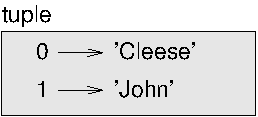
\includegraphics[scale=0.8]{figs/tuple1.pdf}}
\caption{State diagram.}
\label{fig.tuple1}
\end{figure}

But in a larger diagram you might want to leave out the
details.  For example, a diagram of the telephone directory might
appear as in Figure~\ref{fig.dict2}.

在大图中,我们忽略这些细节。 该电话簿的结构图可能像图~\ref{fig.dict2}一样。

\begin{figure}
\centerline
{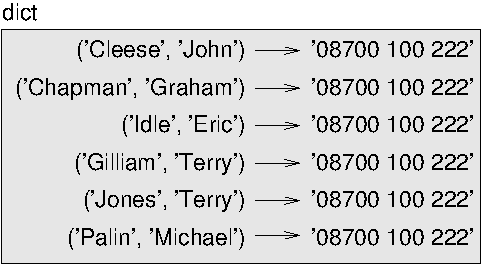
\includegraphics[scale=0.8]{figs/dict2.pdf}}
\caption{State diagram.}
\label{fig.dict2}
\end{figure}

Here the tuples are shown using Python syntax as a graphical
shorthand.  The telephone number in the diagram is the complaints line
for the BBC, so please don't call it.

因此,Python风格的元组用法可用这两幅图来描述。 此图中的电话号码是BBC的投诉热线,请不要拨打它。


\section{Sequences of sequences}
\index{sequence}

I have focused on lists of tuples, but almost all of the examples in
this chapter also work with lists of lists, tuples of tuples, and
tuples of lists.  To avoid enumerating the possible combinations, it
is sometimes easier to talk about sequences of sequences.

In many contexts, the different kinds of sequences (strings, lists and
tuples) can be used interchangeably.  So how should you choose one
over the others?
\index{string}
\index{list}
\index{tuple}
\index{mutability}
\index{immutability}

To start with the obvious, strings are more limited than other
sequences because the elements have to be characters.  They are
also immutable.  If you need the ability to change the characters
in a string (as opposed to creating a new string), you might
want to use a list of characters instead.

Lists are more common than tuples, mostly because they are mutable.
But there are a few cases where you might prefer tuples:

\begin{enumerate}

\item In some contexts, like a {\tt return} statement, it is
syntactically simpler to create a tuple than a list.

\item If you want to use a sequence as a dictionary key, you
have to use an immutable type like a tuple or string.

\item If you are passing a sequence as an argument to a function,
using tuples reduces the potential for unexpected behavior
due to aliasing.

\end{enumerate}

Because tuples are immutable, they don't provide methods like {\tt
  sort} and {\tt reverse}, which modify existing lists.  But Python
provides the built-in function {\tt sorted}, which takes any sequence
and returns a new list with the same elements in sorted order, and
{\tt reversed}, which takes a sequence and returns an iterator that
traverses the list in reverse order.
\index{sorted function}
\index{function!sorted} \index{reversed function}
\index{function!reversed}
\index{iterator}


\section{Debugging}
\index{debugging}
\index{data structure}
\index{shape error}
\index{error!shape}

Lists, dictionaries and tuples are examples of {\bf data
  structures}; in this chapter we are starting to see compound data
structures, like lists of tuples, or dictionaries that contain tuples
as keys and lists as values.  Compound data structures are useful, but
they are prone to what I call {\bf shape errors}; that is, errors
caused when a data structure has the wrong type, size, or structure.
For example, if you are expecting a list with one integer and I
give you a plain old integer (not in a list), it won't work.
\index{structshape module}
\index{module!structshape}

To help debug these kinds of errors, I have written a module
called {\tt structshape} that provides a function, also called
{\tt structshape}, that takes any kind of data structure as
an argument and returns a string that summarizes its shape.
You can download it from \url{http://thinkpython2.com/code/structshape.py}

Here's the result for a simple list:

\begin{lstlisting}
>>> from structshape import structshape
>>> t = [1, 2, 3]
>>> structshape(t)
'list of 3 int'
\end{lstlisting}
%
A fancier program might write ``list of 3 int{\em s}'', but it
was easier not to deal with plurals.  Here's a list of lists:

\begin{lstlisting}
>>> t2 = [[1,2], [3,4], [5,6]]
>>> structshape(t2)
'list of 3 list of 2 int'
\end{lstlisting}
%
If the elements of the list are not the same type,
{\tt structshape} groups them, in order, by type:

\begin{lstlisting}
>>> t3 = [1, 2, 3, 4.0, '5', '6', [7], [8], 9]
>>> structshape(t3)
'list of (3 int, float, 2 str, 2 list of int, int)'
\end{lstlisting}
%
Here's a list of tuples:

\begin{lstlisting}
>>> s = 'abc'
>>> lt = list(zip(t, s))
>>> structshape(lt)
'list of 3 tuple of (int, str)'
\end{lstlisting}
%
And here's a dictionary with 3 items that map integers to strings.

\begin{lstlisting}
>>> d = dict(lt)
>>> structshape(d)
'dict of 3 int->str'
\end{lstlisting}
%
If you are having trouble keeping track of your data structures,
{\tt structshape} can help.


\section{Glossary}

\begin{description}

\item[tuple:] An immutable sequence of elements.

\item[元组:] 一组不可变的元素的序列。
\index{tuple}

\item[tuple assignment:] An assignment with a sequence on the
right side and a tuple of variables on the left.  The right
side is evaluated and then its elements are assigned to the
variables on the left.

\item[元组赋值:]

\index{tuple assignment} \index{assignment!tuple}

\item[gather:] The operation of assembling a variable-length
argument tuple.
\index{gather}

\item[scatter:] The operation of treating a sequence as a list of
arguments.
\index{scatter}

\item[zip object:] The result of calling a built-in function {\tt zip};
an object that iterates through a sequence of tuples.
\index{zip object}
\index{object!zip}

\item[iterator:] An object that can iterate through a sequence, but
which does not provide list operators and methods.
\index{iterator}

\item[data structure:] A collection of related values, often
organized in lists, dictionaries, tuples, etc.
\index{data structure}

\item[shape error:] An error caused because a value has the
wrong shape; that is, the wrong type or size.
\index{shape}

\end{description}


\section{Exercises}

\begin{exercise}

Write a function called \verb"most_frequent" that takes a string and
prints the letters in decreasing order of frequency.  Find text
samples from several different languages and see how letter frequency
varies between languages.  Compare your results with the tables at
\url{http://en.wikipedia.org/wiki/Letter_frequencies}.  Solution:
\url{http://thinkpython2.com/code/most_frequent.py}.  \index{letter
  frequency} \index{frequency!letter}

\end{exercise}


\begin{exercise}
\label{anagrams}
\index{anagram set}
\index{set!anagram}

More anagrams!

\begin{enumerate}

\item Write a program
that reads a word list from a file (see Section~\ref{wordlist}) and
prints all the sets of words that are anagrams.

Here is an example of what the output might look like:

\begin{lstlisting}
['deltas', 'desalt', 'lasted', 'salted', 'slated', 'staled']
['retainers', 'ternaries']
['generating', 'greatening']
['resmelts', 'smelters', 'termless']
\end{lstlisting}
%
Hint: you might want to build a dictionary that maps from a
collection of letters to a list of words that can be spelled with those
letters.  The question is, how can you represent the collection of
letters in a way that can be used as a key?

\item Modify the previous program so that it prints the longest list
of anagrams first, followed by the second longest, and so on.
\index{Scrabble}
\index{bingo}

\item In Scrabble a ``bingo'' is when you play all seven tiles in
your rack, along with a letter on the board, to form an eight-letter
word.  What collection of 8 letters forms the most possible bingos?
Hint: there are seven.

% (7, ['angriest', 'astringe', 'ganister', 'gantries', 'granites',
% 'ingrates', 'rangiest'])

Solution: \url{http://thinkpython2.com/code/anagram_sets.py}.

\end{enumerate}
\end{exercise}

\begin{exercise}
\index{metathesis}

Two words form a ``metathesis pair'' if you can transform one into the
other by swapping two letters; for example, ``converse'' and
``conserve''.  Write a program that finds all of the metathesis pairs
in the dictionary.  Hint: don't test all pairs of words, and don't
test all possible swaps.  Solution:
\url{http://thinkpython2.com/code/metathesis.py}.  Credit: This
exercise is inspired by an example at \url{http://puzzlers.org}.

\end{exercise}


\begin{exercise}
\index{Car Talk}
\index{Puzzler}

Here's another Car Talk Puzzler
(\url{http://www.cartalk.com/content/puzzlers}):

\begin{quote}
What is the longest English word, that remains a valid English word,
as you remove its letters one at a time?

Now, letters can be removed from either end, or the middle, but you
can't rearrange any of the letters. Every time you drop a letter, you
wind up with another English word. If you do that, you're eventually
going to wind up with one letter and that too is going to be an
English word---one that's found in the dictionary. I want to know
what's the longest word and how many letters does it
have?

I'm going to give you a little modest example: Sprite. Ok? You start
off with sprite, you take a letter off, one from the interior of the
word, take the r away, and we're left with the word spite, then we
take the e off the end, we're left with spit, we take the s off, we're
left with pit, it, and I.
\end{quote}
\index{reducible word}
\index{word, reducible}

Write a program to find all words that can be reduced in this way,
and then find the longest one.

This exercise is a little more challenging than most, so here are
some suggestions:

\begin{enumerate}

\item You might want to write a function that takes a word and
  computes a list of all the words that can be formed by removing one
  letter.  These are the ``children'' of the word.
\index{recursive definition}
\index{definition!recursive}

\item Recursively, a word is reducible if any of its children
are reducible.  As a base case, you can consider the empty
string reducible.

\item The wordlist I provided, {\tt words.txt}, doesn't
contain single letter words.  So you might want to add
``I'', ``a'', and the empty string.

\item To improve the performance of your program, you might want
to memoize the words that are known to be reducible.

\end{enumerate}

Solution: \url{http://thinkpython2.com/code/reducible.py}.

\end{exercise}




%\begin{exercise}
%\url{http://en.wikipedia.org/wiki/Word_Ladder}
%\end{exercise}



